\begin{blocksection}
\question
\textbf{bedwars}\\
Fill in each blank in the code example below so that its environment diagram is the following.

\begin{multicols}{2}
\begin{lstlisting}
def bed(wars):
    return lambda iron: ____(____(____) + ____*____)

def hy(pixel):
    ____________
    return _____

________________
____(hy)(pixel)
\end{lstlisting}

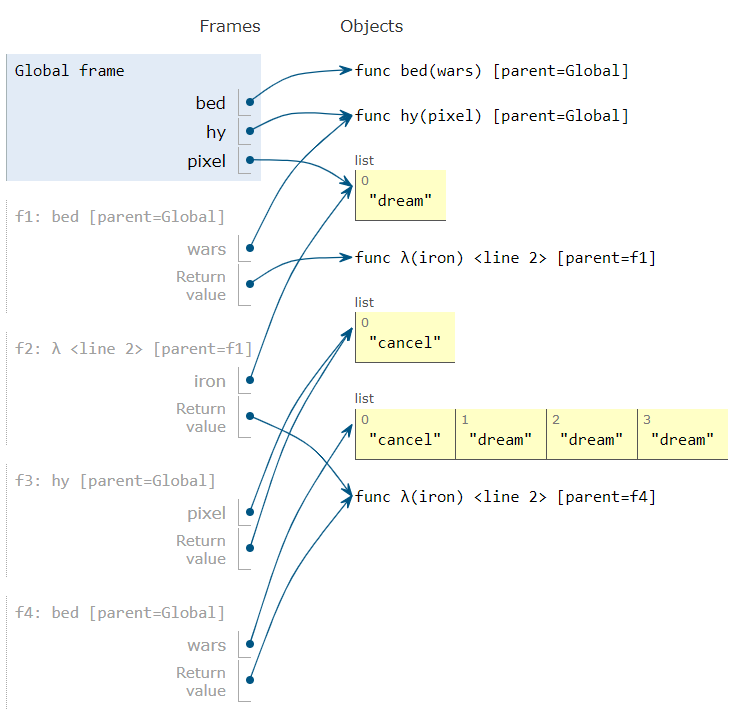
\includegraphics[width=.5\textwidth]{bedwars.png}
\end{multicols}

\begin{solution}[2in]
\begin{lstlisting}
def bed(wars):
    return lambda iron: bed(wars([]) + iron*3)

def hy(pixel):
    pixel = pixel + ['cancel']
    return pixel

pixel=['dream']
bed(hy)(pixel)
\end{lstlisting}
\end{solution}
\end{blocksection}

\begin{blocksection}
\begin{guide}
\textbf{Teaching Tips}
\begin{itemize}
\item Keep track of what exactly the lambda does! It gets trippy since there are so many function calls embedded.
\item Emphasize how we keep creating new lists instead of modifying our existing one inside of \texttt{hy}.
\end{itemize}
\end{guide}
\end{blocksection}
